% !TeX root = ../../main_socg.tex

Because the TCC only confirms coverage of a \emph{superlevel} set $D\setminus B_\omega$, we cannot guarantee coverage of the entire domain.
Indeed, we could compute the persistent homology of the \emph{restriction} of $f$ to the superlevel set we cover in the standard way~\cite{chazal09analysis}.
Instead, we will approximate the persistent homology of the sublevel set filtration \emph{relative to} the sublevel set $B_\omega$.
In the next section we will discuss an interpretation of the relative diagram that is motivated by examples in Section~\ref{sec:experiments}.

\begin{figure}[htbp]
  \centering
  \begin{minipage}[b]{0.27\textwidth}
    
\includegraphics[trim=200 200 200 100, clip, width=\textwidth]{scripts/figures/surf/ass2_C_side.png}\\
    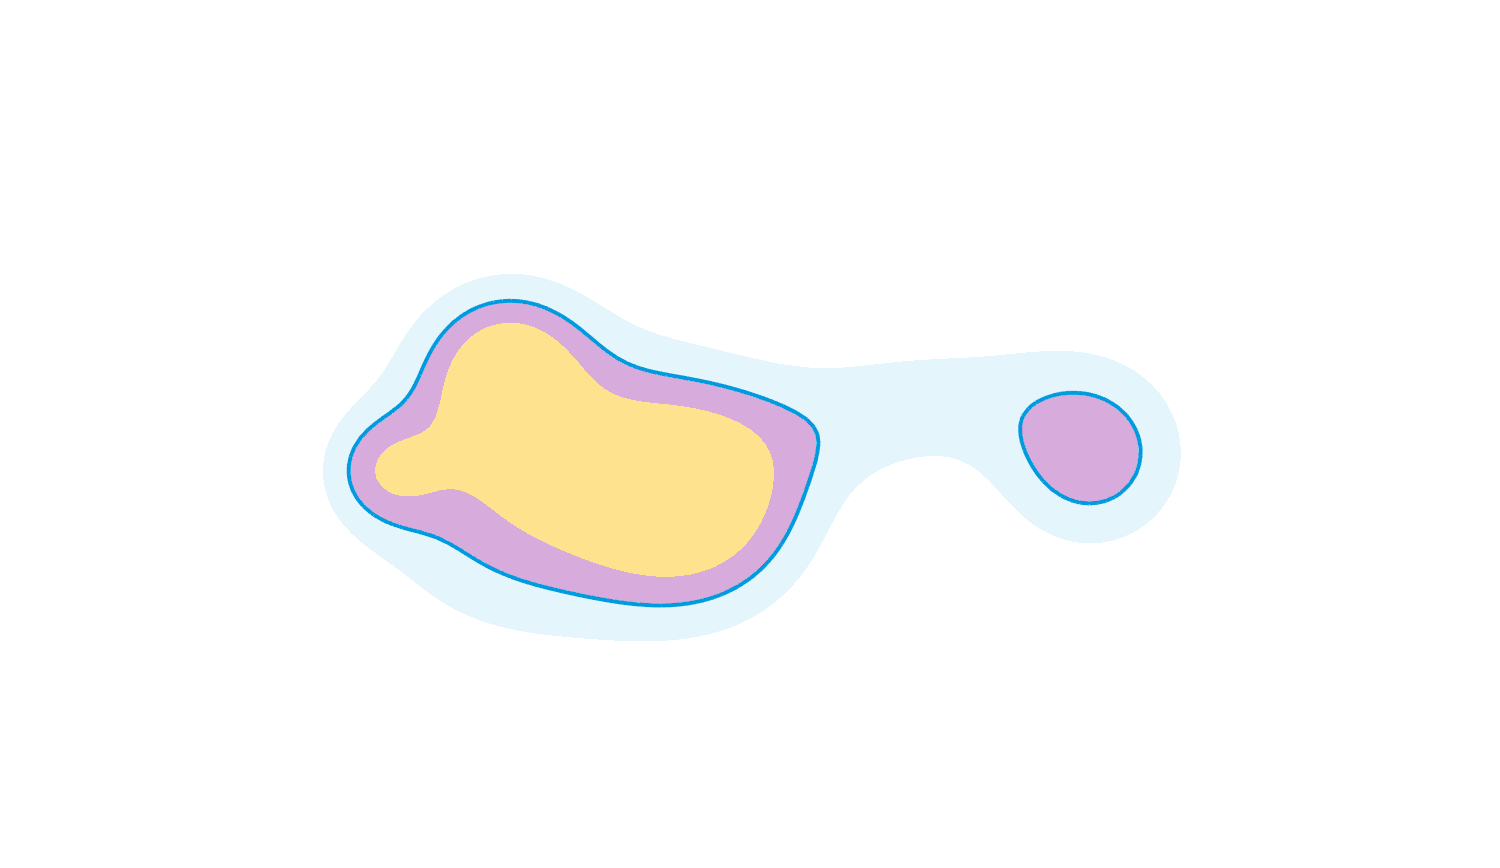
\includegraphics[trim=200 100 200 200, clip, width=\textwidth]{scripts/figures/surf/ass2_C_top.png}
  \end{minipage}
  \begin{minipage}[b]{0.7\textwidth}
    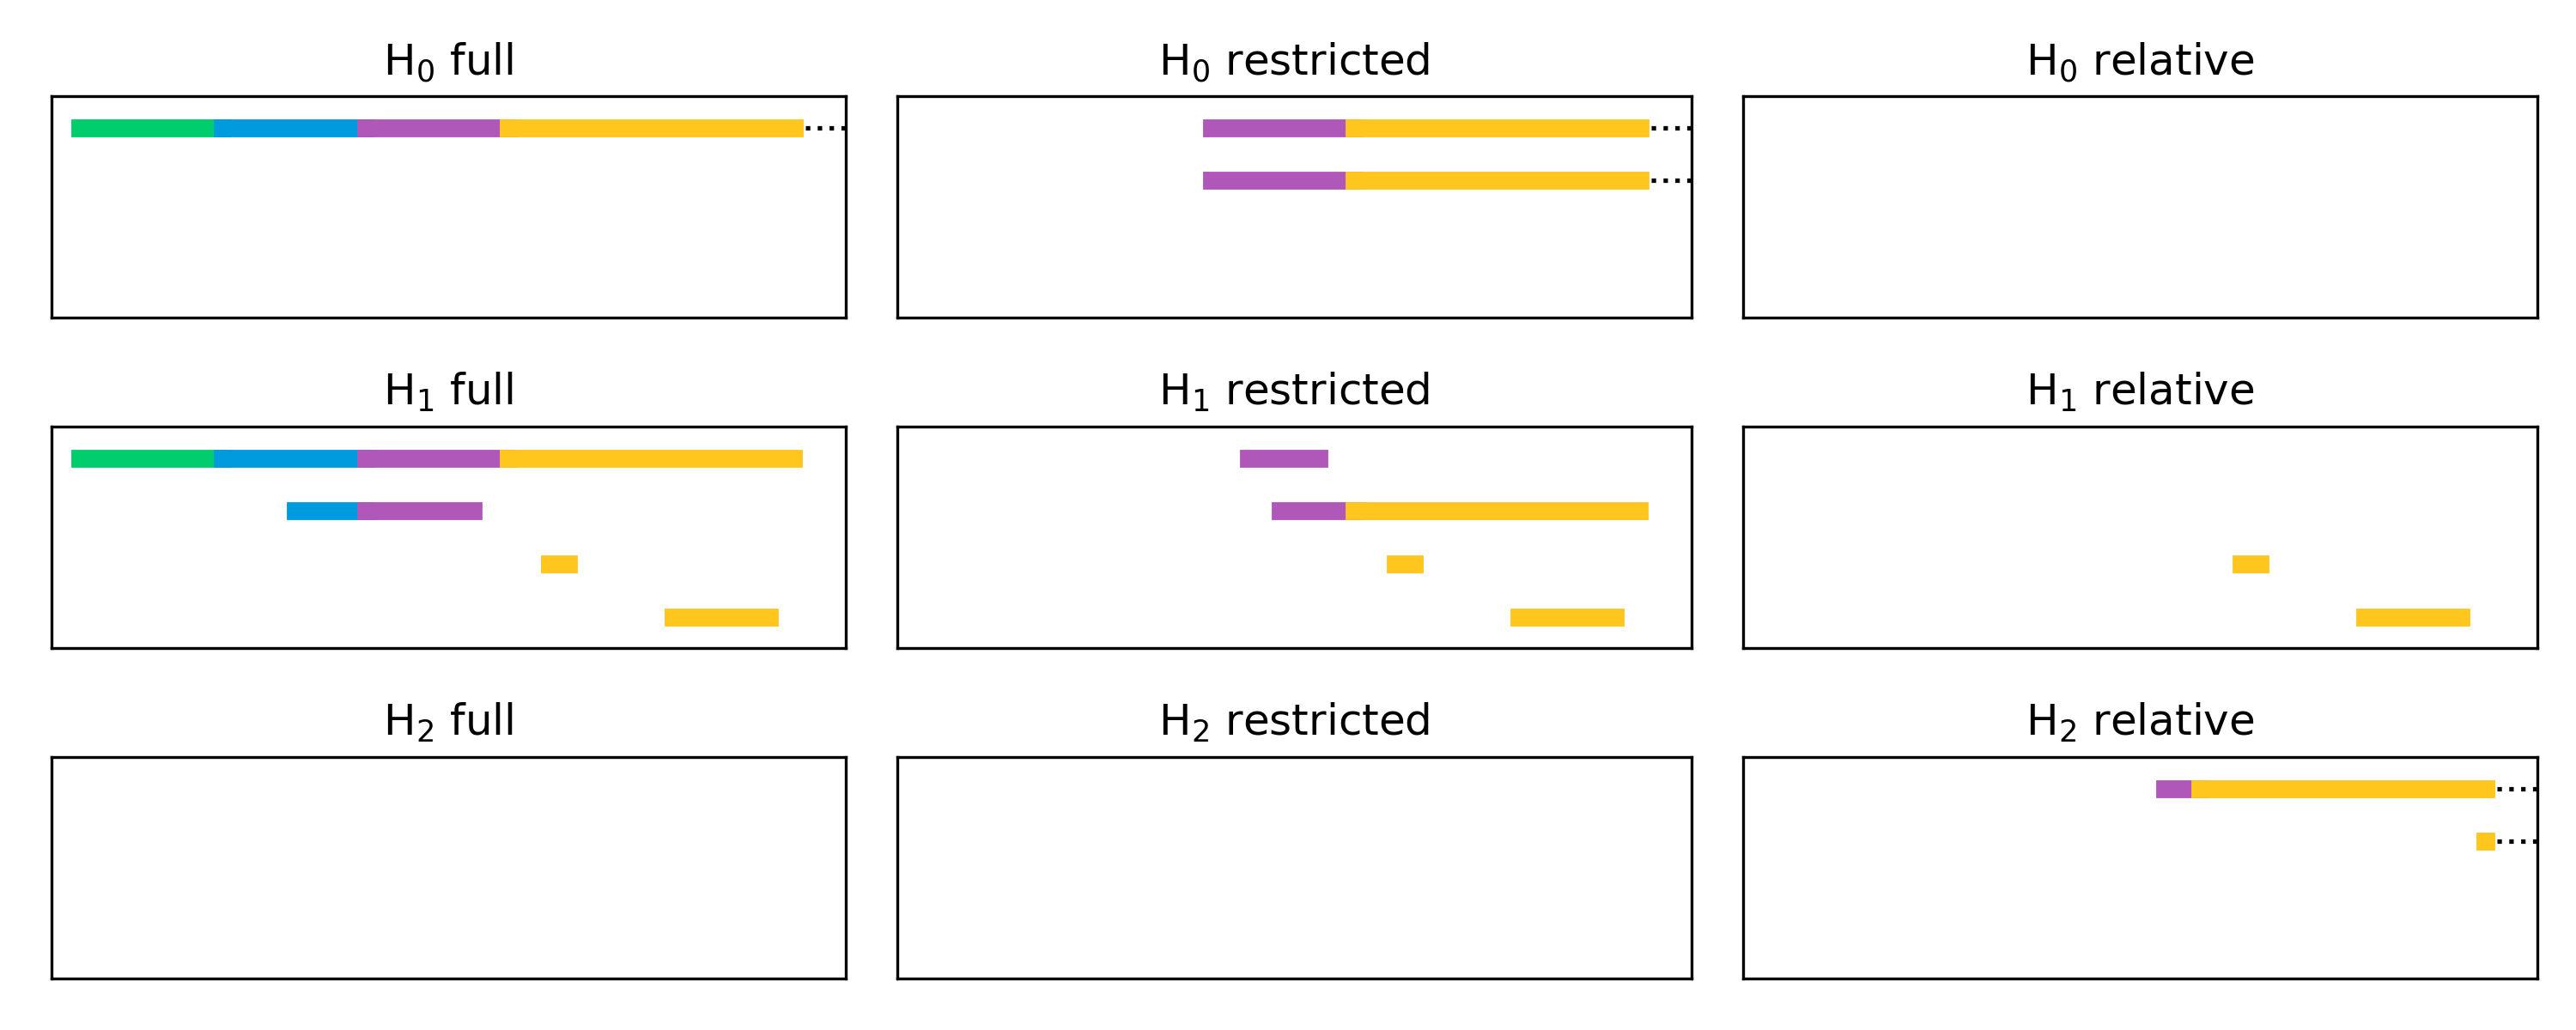
\includegraphics[width=\textwidth]{scripts/figures/barcodes/res_rel.png}
  \end{minipage}
  \caption{Full, restricted, and relative barcodes of the function (left).}% on a $512\times 512$ grid.
    % The restricted barcode is of the function restricted to the region above the blue line.
    % The relative barcode is of the function relative to the blue sub-levelset below the blue line.}
    % We note that the additional features in restricted $\hom_0$ are artifacts of the restriction caused by the approximation.}
\end{figure}

We will first introduce the notion of an extension which will provide us with maps on relative homology induced by inclusion via excision.
However, even then, a map that factors through our pair $(D, B_\omega)$ is not enough to prove an interleaving of persistence modules by inclusion directly.
To address this we impose conditions on sublevel sets near $B_\omega$ which generalize the assumptions made in the TCC.
%  on maps induced by the inclusions
% \[ D\setminus B_{\omega+c(\delta+\zeta)}\hookrightarrow D\setminus B_\omega\hookrightarrow D\setminus B_{\omega-c(\delta+\zeta)}\]
% on $0$-dimensional homology, to assumptions on maps induced by the corresponding inclusions
% \[ B_{\omega-c(\delta+\zeta)}\hookrightarrow B_\omega\hookrightarrow B_{\omega+c(\delta+\zeta)}\]
% on homology in all dimensions $k$.

\subsection{Extensions and Image Persistence Modules}

Suppose $D$ is a subspace of $X$.
We define the extension of a surrounding pair in $D$ to a surrounding pair in $X$ with isomorphic relative homology.

\begin{definition}[Extension]
  If $V$ surrounds $U$ in a subspace $D$ of $X$ let $\ext{V} := V\sqcup (D\setminus U)$ denote the (disjoint) union of the separating set $V$ with the complement of $U$ in $D$.
  The \textbf{extension of $(U, V)$ in $D$} is the pair $(D, \ext{V}) = (U\sqcup (D\setminus U), V\sqcup (D\setminus U)).$
\end{definition}

Lemma~\ref{lem:surround_and_cover} states that we can use these extensions to interleave a pair $(U, V)$ with a sequence of subsets of $(D, B)$.
Lemma~\ref{excision} we can apply excision to the relative homology groups in order to get equivalent maps on homology that are induced by inclusions.
%TODO Proof of these facts, and their extensions to homomorphisms of persistence modules in the next section, can be found in the \fullversion.

\begin{lemma}\label{lem:surround_and_cover}
  Suppose $V$ surrounds $U$ in $D$ and $B'\subseteq B\subset D$.

  If $D\setminus B\subseteq U$ and $U\cap B'\subseteq V\subseteq B'$ then $B'\subseteq \ext{V}\subseteq B$.
\end{lemma}

\begin{lemma}\label{lem:excision}
  Let $(U, V)$ be an open surrounding pair in a subspace $D$ of $X$.

  Then $\hom_k((U\cap A, V)\hookrightarrow (A, \ext{V}))$ is an isomorphism for all $k$ and $A\subseteq D$ with $\ext{V}\subset A$.
\end{lemma}

The TCC uses a nested pair of spaces in order to filter out noise introduced by the sample.
This same technique is used to approximate the persistent homology of a scalar fields~\cite{chazal09analysis}.
As modules, these nested pairs are the images of homomorphisms between homology groups induced by inclusion, which we refer to as image persistence modules.

% \paragraph{Image Persistence Modules}
\begin{definition}[Image Persistence Module]
  The \textbf{image persistence module} of a homomorphism $\Gamma\in\Hom(\U,\V)$ is the family of subspaces $\{\Gamma_\alpha :=\im~\gamma_\alpha\}$ in $\V$ along with linear maps $\{\gamma_\alpha^\beta := v_\alpha^\beta\rest_{\im~\gamma_\alpha} : \Gamma_\alpha\to\Gamma_\beta\}$ and will be denoted by $\im~\Gamma$.
\end{definition}

While we will primarily work with homomorphisms of persistence modules induced by inclusions, in general, defining homomorphisms between images simply as subspaces of the codomain is not sufficient.
Instead, we require that homomorphisms between image modules commute not only with shifts in scale, but also with the functions themselves.

\begin{definition}[Image Module Homomorphism]
  Given $\Gamma\in\Hom(\U,\V)$ and $\Lambda\in\Hom(\S,\T)$ along with $(F,G)\in\Hom^\delta(\U,\S)\times\Hom^\delta(\V,\T)$ let $\Phi(F, G) : \im~\Gamma\to\im~\Lambda$ denote the family of linear maps $\{\phi_\alpha := g_\alpha\rest_{\Gamma_\alpha} : \Gamma_\alpha\to\Lambda_{\alpha+\delta}\}$.
  $\Phi(F, G)$ is an \textbf{image module homomorphism of degree $\delta$} if the following diagram commutes for all $\alpha\leq\beta$.\footnote{We use the notation $\gamma_\alpha[\beta-\alpha] = v_\alpha^\beta\circ\gamma_\alpha$, $\lambda_\alpha[\beta-\alpha] = t_\alpha^\beta\circ\lambda_\alpha$ to denote the composition of homomorphisms between persistence modules and shifts in scale.}
  \begin{equation}\label{dgm:image_homomorphism}
    \begin{tikzcd}[column sep=large]
        U_\alpha\arrow{r}{\gamma_\alpha[\beta-\alpha]}\arrow{d}{f_\alpha} &
      V_\beta\arrow{d}{g_\beta}\\
      %
      S_{\alpha+\delta}\arrow{r}{\lambda_{\alpha+\delta}[\beta-\alpha]} &
      T_{\beta +\delta}
  \end{tikzcd}\end{equation}
  The space of image module homomorphisms of degree $\delta$ between $\im~\Gamma$ and $\im~\Lambda$ will be denoted $\Hom^\delta(\im~\Gamma,\im~\Lambda)$.
\end{definition}
%
% In the following the existence of an image module homomorphism $\Phi(F, G)\in\Hom^\delta(\im~\Gamma, \im~\Lambda)$ where $\Gamma\in\Hom(\U,\V)$ and $\Lambda\in\Hom(\S,\T)$  will imply that $(F,G)\in\Hom^\delta(\U,\S)\times \Hom^\delta(\V,\T)$.
%
%
The composition of image module homomorphisms are image module homomorphisms.
% That is, for $\Phi'(F', G')\in\Hom^\delta(\im~\Gamma, \im~\Lambda)$ and $\Phi(F, G)\in\Hom^{\delta'}(\im~\Lambda, \im~\Lambda')$ the composition of pairs $(F'\circ F, G'\circ G)$ is an image module homomorphism, denoted $\Phi'\circ \Phi\in\Hom^{\delta+\delta'}(\im~\Gamma,\im~\Lambda')$.
Proof of this fact can be found in the \fullversion.

\paragraph*{Partial Interleavings of Image Modules}

Image module homomorphisms introduce a direction to the traditional notion of interleaving.
% That is, given $\Gamma\in\Hom(\U,\V)$ and $\Lambda\in\Hom(\S,\T)$ and $\Phi(F, G)\in\Hom^\delta(\im~\Gamma, \im~\Lambda)$ we consider the case in which there is only a map $\S\to\V$ that commutes.
As we will see, our interleaving via Lemma~\ref{thm:interleaving_main} involves partially interleaving an image module to two other image modules whose composition is isomorphic to our target.

\begin{definition}[Partial Interleaving of Image Modules]
  % Let $\Gamma\in\Hom(\U,\V)$ and $\Lambda\in\Hom(\S,\T)$.
  % $\Phi(F, G)\in\Hom^\delta(\im~\Gamma,\im~\Lambda)$ is a \textbf{left $\delta$-interleaving of image modules} if there exists some $M\in\Hom^\delta(\S,\V)$ such that $\Gamma[2\delta] = M\circ F$.
  % If $\Lambda[2\delta] = G\circ M$ then $\Phi(F, G)$ is a \textbf{right $\delta$-interleaving of image modules}.
  An image module homomorphism $\Phi(F, G)$ is a \textbf{partial $\delta$-interleaving of image modules}, and denoted $\Phi_M(F, G)$, if there exists $M\in\Hom^\delta(\S,\V)$ such that $\Gamma[2\delta] = M\circ F$ and $\Lambda[2\delta] = G\circ M$.
\end{definition}

% For $I\in\Hom^{2\delta}(\U,\V)$ a pair $(F, M)\in \Hom^\delta(\U,\S)\times\Hom^\delta(\S,\V)$ is a said to factor $I$ through $\S$ with degree $\delta$ if $I = M\circ F$.
% Similarly, if $J\in\Hom^{\delta'}(\S,\T)$ a pair $(F,N)\in\Hom^\delta(\U,\S)\times\Hom^\delta(\T,\V)$ is said to factor $I$ through $J$ with degree $\delta$ if $I = N\circ J\circ F$.
% We will often omit the degree when it is clear from context.

% Proof of the following lemma can be found in the appendix.
% Proof of following lemma is straightforward and can be found in the \fullversion.

% uses partial interleavings surrounding a module $\V$ to prove an interleaving of an image module with $\V$.
%TODO Its proof is straightforward and can be found in the \fullversion.
Lemma~\ref{thm:interleaving_main} uses partial interleavings of a map $\Lambda$ with $\U\to\V$ and $\V\to\W$ along with the hypothesis that $\U\to \W$ is isomorphic to $\V$ to interleave $\im~\Lambda$ with $\V$.
When applied, this hypothesis will be satisfied by assumptions on our sublevel set similar to those made in the TCC.

\begin{lemma}\label{thm:interleaving_main}
  Suppose $\Gamma\in\Hom(\U,\V)$, $\Pi\in\Hom(\V,\W)$, and $\Lambda\in\Hom(\S, \T)$.

  If $\Phi_M(F, G)\in\Hom^\delta(\im~\Gamma, \im~\Lambda)$ and $\Psi_G(M, N)\in\Hom^\delta(\im~\Lambda, \im~\Pi)$ are partial $\delta$-interleavings of image modules such that $\Gamma$ is a epimorphism and $\Pi$ is a monomorphism then $\im~\Lambda$ is $\delta$-interleaved with $\V$.
\end{lemma}
